\section{Evaluation}

We evaluate our work in a machine with Intel(R) Xeon (R) CPU E565 2.4GHz in Ubuntu 16.04. 


There are two things to evaluate, the first is the storage overhead. It should be noted that storage overhead for logical back up is not the same as the storage overhead in the DBMS. For example, 64 bits integer should occupy 64 bits in the DBMS, However, in logical backup, integer is stored as string, which means the storage overhead is related to the length of the string. For example, the integer 123456 can occupy 48 bits. In our evaluation, we compute the storage overhead based on the string representation as the logical backup tool mysqldump do.


Since we may want to remove salt, we first need to konw how fast can we generte a new salt. We do experiment with the function in cryptdb code and find that the computation overhead for one salt is about 0.7 us. So this computation overhead is negligible.



We need to know how much time is consumed to do computation in each layer. Also for each strategy, we should give the estimated time overhead for recovery, so we should know how time is consumed for each algorithm, and we give uses the choice of each strategy. So, our strategy is to show customers the reencryption overhead. 


\begin{figure}[tb]
\centering
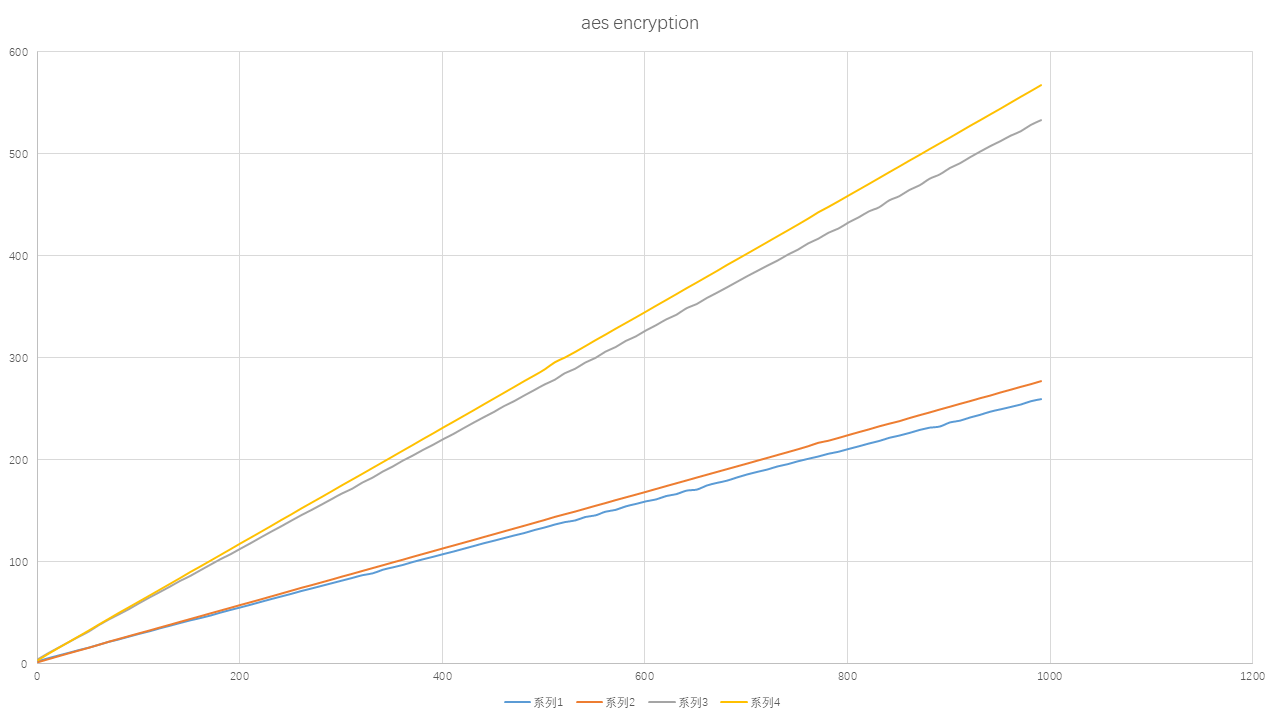
\includegraphics[width=4cm]{images/aes.png}
\caption{Aes time consumpation}
\label{fig:stack9}
\end{figure}


\begin{figure}[tb]
\centering
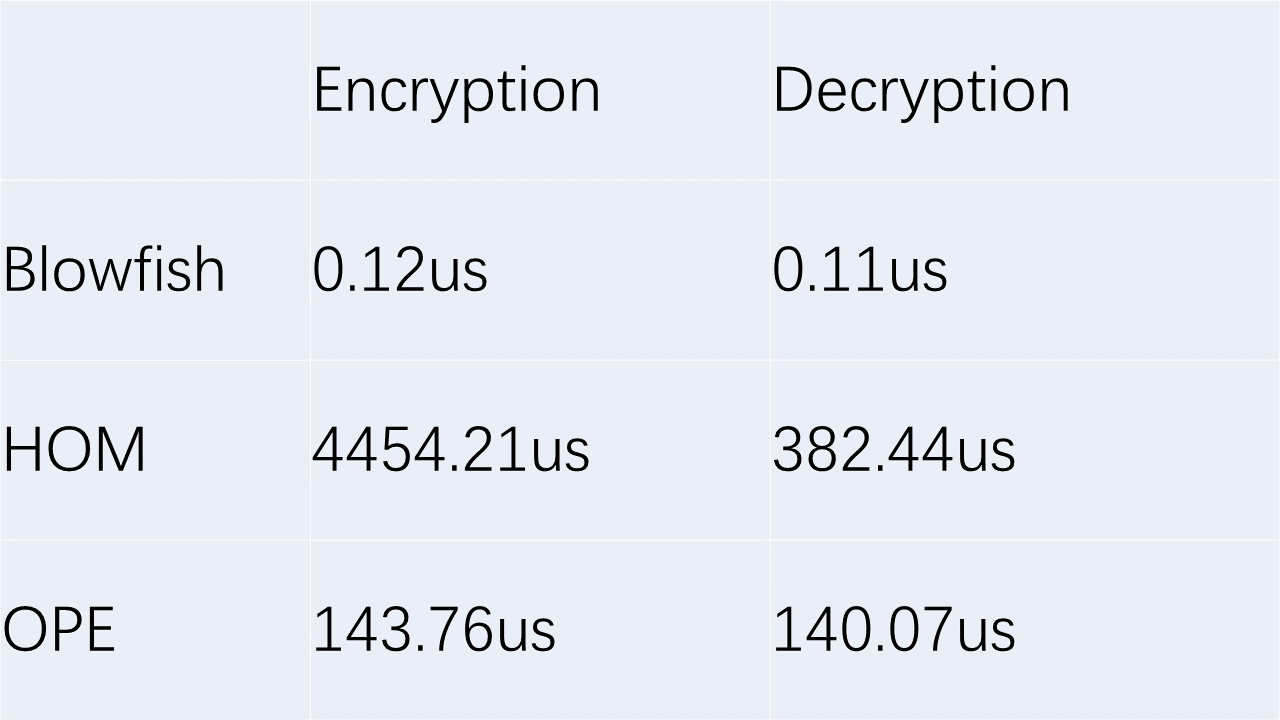
\includegraphics[width=4cm]{images/time.png}
\caption{time consumpation}
\label{fig:stack10}
\end{figure}

As we can see in Figure~\ref{fig:stack9} , we can now estimate the time overhead for each strategy and give suggesstions.


We now begin to analysis the two type of data that is supported by cryptedb.

For integer, as we mentioned before, the column are replicated three onions with an additional salt column. We create one simple table with only one field, and backup based on that data, and show the size of each column.


\begin{figure}[tb]
\centering
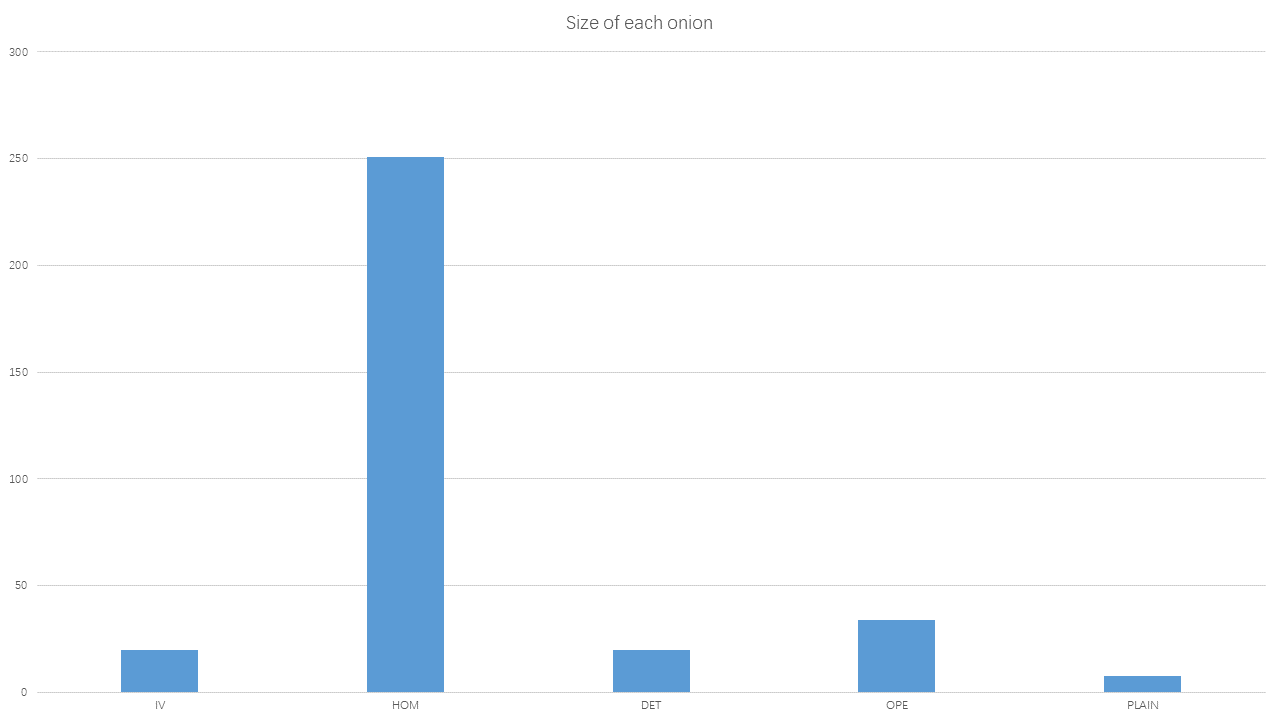
\includegraphics[width=4cm]{images/sizeofeachonion.png}
\caption{Size of onion for integer type}
\label{fig:stack11}
\end{figure}

Figure~\ref{fig:stack11} shows the strategy and the time overhead for each of the strategy we discussed in the string.


For string type, we do experiment with a simple table of varchar(10). After encryption, the onion DET will be tranformed to varbinary(48) due to the padding, and OPE will be varbinary(32), salt should be big int. We insert 1000000 plaintext of length 10 into the table, and the the following results. 


\begin{figure}[tb]
\centering
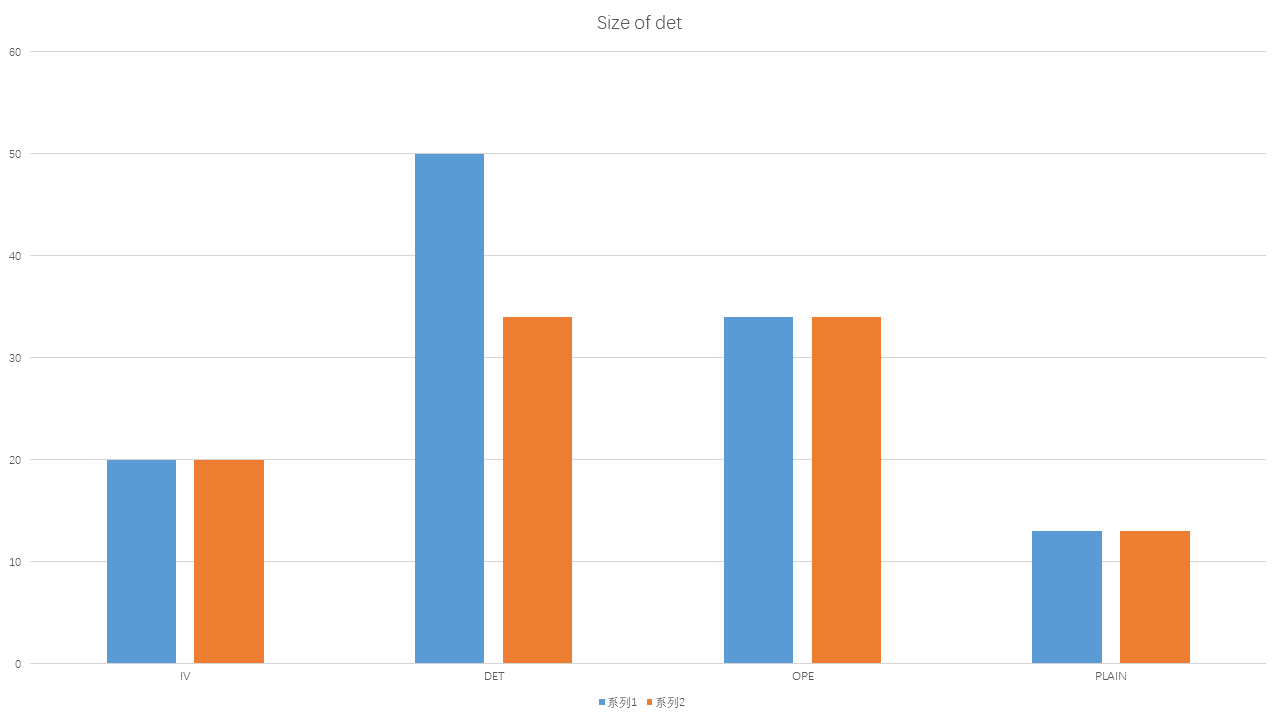
\includegraphics[width=4cm]{images/sizeofstr.png}
\caption{size of onion for string type}
\label{fig:stack12}
\end{figure}


We can find that even for very short string, three layer of encryption in det can make it larger than the onion OPE. So ope is always assumed  smaller than DET. and the size of sat remains the same.


We insert TPC-C data into Cryptdb, and use mysqldump to backup data into a file dump1.sql Then we apply the strategy to the backup process, backup data into a second file dump2.sql, and compare the size of dump1.sql and dump2.sql. We also construct microbenchmark that create table with only string type and integer type.



\begin{figure}[tb]
\centering
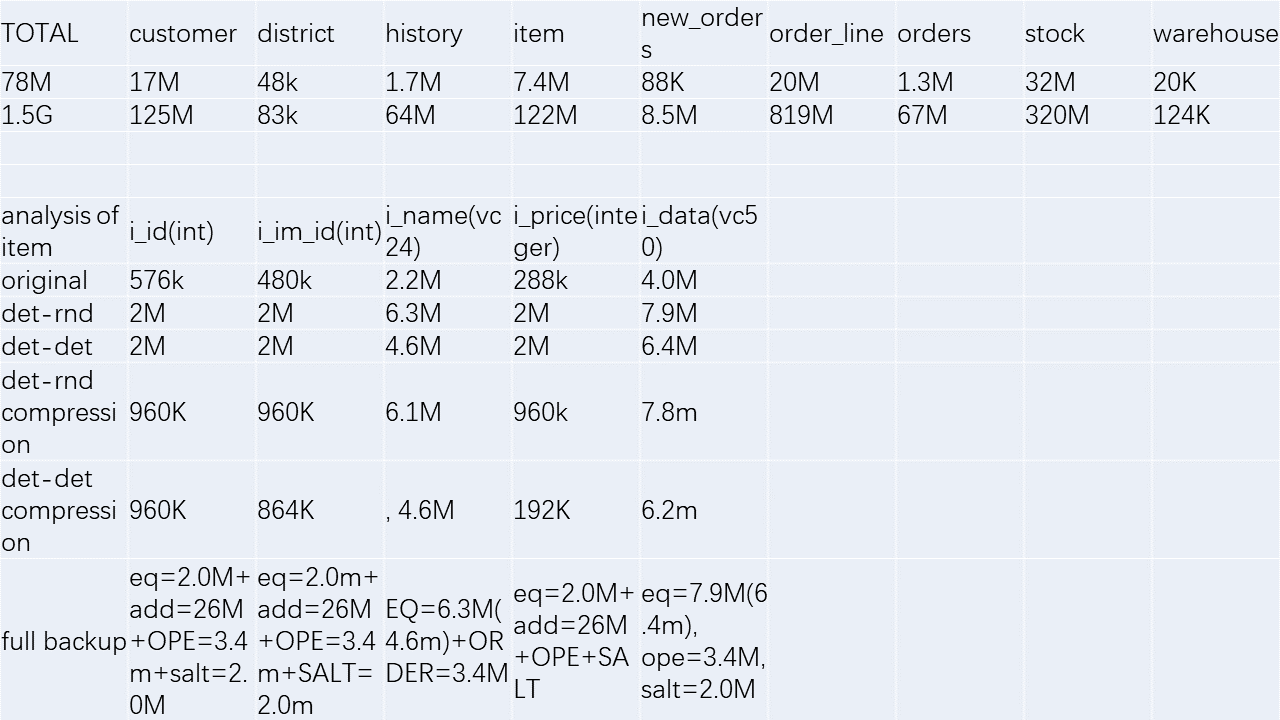
\includegraphics[width=8cm]{images/tpcc.png}
\caption{tpcc data}
\label{fig:stack13}
\end{figure}


DET is always retained. Based on this, we can estimate the overhead for each strategy. 



In this experiment, Cryptdump only dump DET and IV, so for integer type, we can significantly reduce the amount of storage size. We do not use extended insert, so the command we use to backup data is.


mysqldump --skip-extended-insert -uroot -pletmein -h127.0.0.1 --hex-blob --compact tpcc1000 > back.sql



Recovery time is affected by the implementation details. Here we measure the time for the deduplicated data to be recovered to the original data, and this can be considered as the time overhead for recovery.A fter that, we can use the data for backup.


The following we use tpcc to analysis the three main strategy.


Based on the above analysis on the decryption and encryption time, we can conclude that HOM takes longer time for recovery and also has large storage size. So If we need small storage size, we can choose to remove HOM Onion, whlie having long recovery time. On the other hand, If we do not care about storage size, then we can choose to keep Hom onion. 

